% Options for packages loaded elsewhere
\PassOptionsToPackage{unicode}{hyperref}
\PassOptionsToPackage{hyphens}{url}
\PassOptionsToPackage{dvipsnames,svgnames,x11names}{xcolor}
%
\documentclass[
  letterpaper,
  DIV=11,
  numbers=noendperiod]{scrreprt}

\usepackage{amsmath,amssymb}
\usepackage{iftex}
\ifPDFTeX
  \usepackage[T1]{fontenc}
  \usepackage[utf8]{inputenc}
  \usepackage{textcomp} % provide euro and other symbols
\else % if luatex or xetex
  \usepackage{unicode-math}
  \defaultfontfeatures{Scale=MatchLowercase}
  \defaultfontfeatures[\rmfamily]{Ligatures=TeX,Scale=1}
\fi
\usepackage{lmodern}
\ifPDFTeX\else  
    % xetex/luatex font selection
\fi
% Use upquote if available, for straight quotes in verbatim environments
\IfFileExists{upquote.sty}{\usepackage{upquote}}{}
\IfFileExists{microtype.sty}{% use microtype if available
  \usepackage[]{microtype}
  \UseMicrotypeSet[protrusion]{basicmath} % disable protrusion for tt fonts
}{}
\makeatletter
\@ifundefined{KOMAClassName}{% if non-KOMA class
  \IfFileExists{parskip.sty}{%
    \usepackage{parskip}
  }{% else
    \setlength{\parindent}{0pt}
    \setlength{\parskip}{6pt plus 2pt minus 1pt}}
}{% if KOMA class
  \KOMAoptions{parskip=half}}
\makeatother
\usepackage{xcolor}
\setlength{\emergencystretch}{3em} % prevent overfull lines
\setcounter{secnumdepth}{2}
% Make \paragraph and \subparagraph free-standing
\ifx\paragraph\undefined\else
  \let\oldparagraph\paragraph
  \renewcommand{\paragraph}[1]{\oldparagraph{#1}\mbox{}}
\fi
\ifx\subparagraph\undefined\else
  \let\oldsubparagraph\subparagraph
  \renewcommand{\subparagraph}[1]{\oldsubparagraph{#1}\mbox{}}
\fi

\usepackage{color}
\usepackage{fancyvrb}
\newcommand{\VerbBar}{|}
\newcommand{\VERB}{\Verb[commandchars=\\\{\}]}
\DefineVerbatimEnvironment{Highlighting}{Verbatim}{commandchars=\\\{\}}
% Add ',fontsize=\small' for more characters per line
\usepackage{framed}
\definecolor{shadecolor}{RGB}{241,243,245}
\newenvironment{Shaded}{\begin{snugshade}}{\end{snugshade}}
\newcommand{\AlertTok}[1]{\textcolor[rgb]{0.68,0.00,0.00}{#1}}
\newcommand{\AnnotationTok}[1]{\textcolor[rgb]{0.37,0.37,0.37}{#1}}
\newcommand{\AttributeTok}[1]{\textcolor[rgb]{0.40,0.45,0.13}{#1}}
\newcommand{\BaseNTok}[1]{\textcolor[rgb]{0.68,0.00,0.00}{#1}}
\newcommand{\BuiltInTok}[1]{\textcolor[rgb]{0.00,0.23,0.31}{#1}}
\newcommand{\CharTok}[1]{\textcolor[rgb]{0.13,0.47,0.30}{#1}}
\newcommand{\CommentTok}[1]{\textcolor[rgb]{0.37,0.37,0.37}{#1}}
\newcommand{\CommentVarTok}[1]{\textcolor[rgb]{0.37,0.37,0.37}{\textit{#1}}}
\newcommand{\ConstantTok}[1]{\textcolor[rgb]{0.56,0.35,0.01}{#1}}
\newcommand{\ControlFlowTok}[1]{\textcolor[rgb]{0.00,0.23,0.31}{#1}}
\newcommand{\DataTypeTok}[1]{\textcolor[rgb]{0.68,0.00,0.00}{#1}}
\newcommand{\DecValTok}[1]{\textcolor[rgb]{0.68,0.00,0.00}{#1}}
\newcommand{\DocumentationTok}[1]{\textcolor[rgb]{0.37,0.37,0.37}{\textit{#1}}}
\newcommand{\ErrorTok}[1]{\textcolor[rgb]{0.68,0.00,0.00}{#1}}
\newcommand{\ExtensionTok}[1]{\textcolor[rgb]{0.00,0.23,0.31}{#1}}
\newcommand{\FloatTok}[1]{\textcolor[rgb]{0.68,0.00,0.00}{#1}}
\newcommand{\FunctionTok}[1]{\textcolor[rgb]{0.28,0.35,0.67}{#1}}
\newcommand{\ImportTok}[1]{\textcolor[rgb]{0.00,0.46,0.62}{#1}}
\newcommand{\InformationTok}[1]{\textcolor[rgb]{0.37,0.37,0.37}{#1}}
\newcommand{\KeywordTok}[1]{\textcolor[rgb]{0.00,0.23,0.31}{#1}}
\newcommand{\NormalTok}[1]{\textcolor[rgb]{0.00,0.23,0.31}{#1}}
\newcommand{\OperatorTok}[1]{\textcolor[rgb]{0.37,0.37,0.37}{#1}}
\newcommand{\OtherTok}[1]{\textcolor[rgb]{0.00,0.23,0.31}{#1}}
\newcommand{\PreprocessorTok}[1]{\textcolor[rgb]{0.68,0.00,0.00}{#1}}
\newcommand{\RegionMarkerTok}[1]{\textcolor[rgb]{0.00,0.23,0.31}{#1}}
\newcommand{\SpecialCharTok}[1]{\textcolor[rgb]{0.37,0.37,0.37}{#1}}
\newcommand{\SpecialStringTok}[1]{\textcolor[rgb]{0.13,0.47,0.30}{#1}}
\newcommand{\StringTok}[1]{\textcolor[rgb]{0.13,0.47,0.30}{#1}}
\newcommand{\VariableTok}[1]{\textcolor[rgb]{0.07,0.07,0.07}{#1}}
\newcommand{\VerbatimStringTok}[1]{\textcolor[rgb]{0.13,0.47,0.30}{#1}}
\newcommand{\WarningTok}[1]{\textcolor[rgb]{0.37,0.37,0.37}{\textit{#1}}}

\providecommand{\tightlist}{%
  \setlength{\itemsep}{0pt}\setlength{\parskip}{0pt}}\usepackage{longtable,booktabs,array}
\usepackage{calc} % for calculating minipage widths
% Correct order of tables after \paragraph or \subparagraph
\usepackage{etoolbox}
\makeatletter
\patchcmd\longtable{\par}{\if@noskipsec\mbox{}\fi\par}{}{}
\makeatother
% Allow footnotes in longtable head/foot
\IfFileExists{footnotehyper.sty}{\usepackage{footnotehyper}}{\usepackage{footnote}}
\makesavenoteenv{longtable}
\usepackage{graphicx}
\makeatletter
\def\maxwidth{\ifdim\Gin@nat@width>\linewidth\linewidth\else\Gin@nat@width\fi}
\def\maxheight{\ifdim\Gin@nat@height>\textheight\textheight\else\Gin@nat@height\fi}
\makeatother
% Scale images if necessary, so that they will not overflow the page
% margins by default, and it is still possible to overwrite the defaults
% using explicit options in \includegraphics[width, height, ...]{}
\setkeys{Gin}{width=\maxwidth,height=\maxheight,keepaspectratio}
% Set default figure placement to htbp
\makeatletter
\def\fps@figure{htbp}
\makeatother

% Soul package to handle highlighting (see hl.py3 filter)
\usepackage{soul}

% For tables generated by the gt package
\usepackage{colortbl}
\KOMAoption{captions}{tableheading}
\makeatletter
\@ifpackageloaded{bookmark}{}{\usepackage{bookmark}}
\makeatother
\makeatletter
\@ifpackageloaded{caption}{}{\usepackage{caption}}
\AtBeginDocument{%
\ifdefined\contentsname
  \renewcommand*\contentsname{Índice}
\else
  \newcommand\contentsname{Índice}
\fi
\ifdefined\listfigurename
  \renewcommand*\listfigurename{Lista de Figuras}
\else
  \newcommand\listfigurename{Lista de Figuras}
\fi
\ifdefined\listtablename
  \renewcommand*\listtablename{Lista de Tabelas}
\else
  \newcommand\listtablename{Lista de Tabelas}
\fi
\ifdefined\figurename
  \renewcommand*\figurename{Figura}
\else
  \newcommand\figurename{Figura}
\fi
\ifdefined\tablename
  \renewcommand*\tablename{Tabela}
\else
  \newcommand\tablename{Tabela}
\fi
}
\@ifpackageloaded{float}{}{\usepackage{float}}
\floatstyle{ruled}
\@ifundefined{c@chapter}{\newfloat{codelisting}{h}{lop}}{\newfloat{codelisting}{h}{lop}[chapter]}
\floatname{codelisting}{Listagem}
\newcommand*\listoflistings{\listof{codelisting}{Lista de Listagens}}
\makeatother
\makeatletter
\makeatother
\makeatletter
\@ifpackageloaded{caption}{}{\usepackage{caption}}
\@ifpackageloaded{subcaption}{}{\usepackage{subcaption}}
\makeatother
\ifLuaTeX
\usepackage[bidi=basic]{babel}
\else
\usepackage[bidi=default]{babel}
\fi
\babelprovide[main,import]{portuguese}
% get rid of language-specific shorthands (see #6817):
\let\LanguageShortHands\languageshorthands
\def\languageshorthands#1{}
\ifLuaTeX
  \usepackage{selnolig}  % disable illegal ligatures
\fi
\usepackage{bookmark}

\IfFileExists{xurl.sty}{\usepackage{xurl}}{} % add URL line breaks if available
\urlstyle{same} % disable monospaced font for URLs
\hypersetup{
  pdftitle={Comparando listas e rankings},
  pdfauthor={Fernando Náufel},
  pdflang={pt},
  colorlinks=true,
  linkcolor={blue},
  filecolor={Maroon},
  citecolor={Blue},
  urlcolor={Blue},
  pdfcreator={LaTeX via pandoc}}

\title{Comparando listas e rankings}
\author{Fernando Náufel}
\date{09/02/2024 19:40}

\begin{document}
\maketitle

% Bold title in callout boxes
% But we must be careful: if there are no callout boxes in the document,
% then package tcolorbox has NOT been loaded, and we must refrain from
% setting this up; hence the ifpackageloaded
\makeatletter
\@ifpackageloaded{tcolorbox}
{\tcbset{fonttitle=\bfseries}}
{}
\makeatother


\renewcommand*\contentsname{Índice}
{
\hypersetup{linkcolor=}
\setcounter{tocdepth}{2}
\tableofcontents
}
\bookmarksetup{startatroot}

\chapter*{Apresentação}\label{apresentauxe7uxe3o}
\addcontentsline{toc}{chapter}{Apresentação}

\markboth{Apresentação}{Apresentação}

???

\bookmarksetup{startatroot}

\chapter{\texorpdfstring{Gerar e visualizar
\emph{rankings}}{Gerar e visualizar rankings}}\label{gerar-e-visualizar-rankings}

\section{Problema}\label{problema}

Vamos trabalhar com listas e \emph{rankings} sujeitos às seguintes
condições:

\begin{itemize}
\item
  A {\hl{lista}} tem $k$ elementos, $k > 0$, {\hl{não ordenados}}.
\item
  O {\hl{\emph{ranking}}} tem $p$ elementos, $p \geq k$,
  {\hl{ordenados}}, {\hl{sem empates}}.
\item
  Todos os elementos da lista estão no \emph{ranking}.
\item
  O último elemento do \emph{ranking} é elemento da lista.
\item
  As identidades dos elementos do \emph{ranking} não importam --- i.e.,
  eles são indistinguíveis, a não ser por pertencerem ou não à lista (e
  pela ordem que ocupam no \emph{ranking}, claro).
\end{itemize}

\section{\texorpdfstring{Criando
\emph{rankings}}{Criando rankings}}\label{criando-rankings}

\subsection{\texorpdfstring{Quantidade de
\emph{rankings}}{Quantidade de rankings}}\label{quantidade-de-rankings}

Dados $k > 0$ e $p \geq k$ fixos, quantos \emph{rankings} existem?

Para montar um \emph{ranking}:

\begin{enumerate}
\def\labelenumi{\arabic{enumi}.}
\item
  Sabemos que a última posição é ocupada por alguém da lista.
\item
  Só resta escolher as posições dos $k - 1$ elementos restantes da lista
  dentre as $p - 1$ posições restantes no \emph{ranking}, o que dá
  $\binom{p - 1}{k - 1}$ escolhas.
\end{enumerate}

Assim, a quantidade total de \emph{rankings} para $k$ e $p$ dados é

\[
\binom{p - 1}{k - 1}
\]

\subsection{Representação}\label{sec-repr}

Considere naturais $k > 0$ e $p \geq k$.

{\hl{Podemos representar um \emph{ranking} através de um \emph{string}
contendo $k$ caracteres ``{\mbox{\texttt{x}}}'' e $p - k$ caracteres
``{\mbox{\texttt{-}}}''}}.

``\texttt{x}'' representa uma posição ocupada por um elemento da lista.

``\texttt{-}'' representa uma posição ocupada por um elemento que não
está na lista.

Por exemplo, para $k = 3, p = 5$, os $\binom{4}{2} = 6$ \emph{rankings}
possíveis são

\begin{itemize}
\tightlist
\item
  \texttt{xx-\/-x}
\item
  \texttt{x-x-x}
\item
  \texttt{x-\/-xx}
\item
  \texttt{-xx-x}
\item
  \texttt{-x-xx}
\item
  \texttt{-\/-xxx}
\end{itemize}

A tabela a seguir (na verdade, um pedaço do triângulo de Pascal) mostra
as quantidades de \emph{rankings} possíveis para alguns valores de $k$ e
$p$:

\begin{longtable*}{l|rrrrrrrrrr}
\toprule
\multicolumn{1}{l}{} & \multicolumn{10}{c}{\(k\)} \\ 
\cmidrule(lr){2-11}
\multicolumn{1}{l}{\(p\)} & 1 & 2 & 3 & 4 & 5 & 6 & 7 & 8 & 9 & 10 \\ 
\midrule\addlinespace[2.5pt]
$1$ & $1$ &  &  &  &  &  &  &  &  &  \\ 
$2$ & $1$ & $1$ &  &  &  &  &  &  &  &  \\ 
$3$ & $1$ & $2$ & $1$ &  &  &  &  &  &  &  \\ 
$4$ & $1$ & $3$ & $3$ & $1$ &  &  &  &  &  &  \\ 
$5$ & $1$ & $4$ & $6$ & $4$ & $1$ &  &  &  &  &  \\ 
$6$ & $1$ & $5$ & $10$ & $10$ & $5$ & $1$ &  &  &  &  \\ 
$7$ & $1$ & $6$ & $15$ & $20$ & $15$ & $6$ & $1$ &  &  &  \\ 
$8$ & $1$ & $7$ & $21$ & $35$ & $35$ & $21$ & $7$ & $1$ &  &  \\ 
$9$ & $1$ & $8$ & $28$ & $56$ & $70$ & $56$ & $28$ & $8$ & $1$ &  \\ 
$10$ & $1$ & $9$ & $36$ & $84$ & $126$ & $126$ & $84$ & $36$ & $9$ & $1$ \\ 
$11$ & $1$ & $10$ & $45$ & $120$ & $210$ & $252$ & $210$ & $120$ & $45$ & $10$ \\ 
$12$ & $1$ & $11$ & $55$ & $165$ & $330$ & $462$ & $462$ & $330$ & $165$ & $55$ \\ 
$13$ & $1$ & $12$ & $66$ & $220$ & $495$ & $792$ & $924$ & $792$ & $495$ & $220$ \\ 
$14$ & $1$ & $13$ & $78$ & $286$ & $715$ & $1.287$ & $1.716$ & $1.716$ & $1.287$ & $715$ \\ 
$15$ & $1$ & $14$ & $91$ & $364$ & $1.001$ & $2.002$ & $3.003$ & $3.432$ & $3.003$ & $2.002$ \\ 
$16$ & $1$ & $15$ & $105$ & $455$ & $1.365$ & $3.003$ & $5.005$ & $6.435$ & $6.435$ & $5.005$ \\ 
$17$ & $1$ & $16$ & $120$ & $560$ & $1.820$ & $4.368$ & $8.008$ & $11.440$ & $12.870$ & $11.440$ \\ 
$18$ & $1$ & $17$ & $136$ & $680$ & $2.380$ & $6.188$ & $12.376$ & $19.448$ & $24.310$ & $24.310$ \\ 
$19$ & $1$ & $18$ & $153$ & $816$ & $3.060$ & $8.568$ & $18.564$ & $31.824$ & $43.758$ & $48.620$ \\ 
$20$ & $1$ & $19$ & $171$ & $969$ & $3.876$ & $11.628$ & $27.132$ & $50.388$ & $75.582$ & $92.378$ \\ 
$21$ & $1$ & $20$ & $190$ & $1.140$ & $4.845$ & $15.504$ & $38.760$ & $77.520$ & $125.970$ & $167.960$ \\ 
$22$ & $1$ & $21$ & $210$ & $1.330$ & $5.985$ & $20.349$ & $54.264$ & $116.280$ & $203.490$ & $293.930$ \\ 
$23$ & $1$ & $22$ & $231$ & $1.540$ & $7.315$ & $26.334$ & $74.613$ & $170.544$ & $319.770$ & $497.420$ \\ 
$24$ & $1$ & $23$ & $253$ & $1.771$ & $8.855$ & $33.649$ & $100.947$ & $245.157$ & $490.314$ & $817.190$ \\ 
$25$ & $1$ & $24$ & $276$ & $2.024$ & $10.626$ & $42.504$ & $134.596$ & $346.104$ & $735.471$ & $1.307.504$ \\ 
$26$ & $1$ & $25$ & $300$ & $2.300$ & $12.650$ & $53.130$ & $177.100$ & $480.700$ & $1.081.575$ & $2.042.975$ \\ 
$27$ & $1$ & $26$ & $325$ & $2.600$ & $14.950$ & $65.780$ & $230.230$ & $657.800$ & $1.562.275$ & $3.124.550$ \\ 
$28$ & $1$ & $27$ & $351$ & $2.925$ & $17.550$ & $80.730$ & $296.010$ & $888.030$ & $2.220.075$ & $4.686.825$ \\ 
$29$ & $1$ & $28$ & $378$ & $3.276$ & $20.475$ & $98.280$ & $376.740$ & $1.184.040$ & $3.108.105$ & $6.906.900$ \\ 
$30$ & $1$ & $29$ & $406$ & $3.654$ & $23.751$ & $118.755$ & $475.020$ & $1.560.780$ & $4.292.145$ & $10.015.005$ \\ 
\bottomrule
\end{longtable*}

\subsection{\texorpdfstring{Criar um \emph{ranking} a partir de um
vetor}{Criar um ranking a partir de um vetor}}\label{criar-um-ranking-a-partir-de-um-vetor}

Em vez de especificar as $p$ posições do \emph{ranking}, {\hl{pode ser
mais compacto especificar as $k$ posições do \emph{ranking} que são
ocupadas por elementos da lista}}.

A função \texttt{rk()} faz isso, recebendo um vetor numérico com $k$
elementos e retornando um \emph{string}.

\begin{Shaded}
\begin{Highlighting}[]
\NormalTok{rk }\OtherTok{\textless{}{-}} \ControlFlowTok{function}\NormalTok{(v) \{}
  
\NormalTok{  k }\OtherTok{\textless{}{-}} \FunctionTok{length}\NormalTok{(v)}
\NormalTok{  p }\OtherTok{\textless{}{-}} \FunctionTok{max}\NormalTok{(v)   }\CommentTok{\# o último elemento pertence à lista}
  
  \CommentTok{\# Verificar se posicoes contêm só números entre 1 e p, sem repetições}
  \FunctionTok{stopifnot}\NormalTok{(}
    \StringTok{\textquotesingle{}Valores precisam ser inteiros positivos, sem repetições.\textquotesingle{}} \OtherTok{=}
    \FunctionTok{all}\NormalTok{(v }\SpecialCharTok{==} \FunctionTok{as.integer}\NormalTok{(v)) }\SpecialCharTok{\&} 
      \FunctionTok{all}\NormalTok{(v }\SpecialCharTok{\textgreater{}} \DecValTok{0}\NormalTok{) }\SpecialCharTok{\&}
      \FunctionTok{identical}\NormalTok{(v, }\FunctionTok{unique}\NormalTok{(v))}
\NormalTok{  )}

\NormalTok{  s }\OtherTok{\textless{}{-}} \FunctionTok{rep}\NormalTok{(}\StringTok{\textquotesingle{}{-}\textquotesingle{}}\NormalTok{, p)}
\NormalTok{  s[v] }\OtherTok{\textless{}{-}} \StringTok{\textquotesingle{}x\textquotesingle{}}
  
  \FunctionTok{paste0}\NormalTok{(s, }\AttributeTok{collapse =} \StringTok{\textquotesingle{}\textquotesingle{}}\NormalTok{)}
  
\NormalTok{\}}
\end{Highlighting}
\end{Shaded}

\begin{Shaded}
\begin{Highlighting}[]
\FunctionTok{rk}\NormalTok{(}\FunctionTok{c}\NormalTok{(}\DecValTok{1}\NormalTok{, }\DecValTok{3}\NormalTok{, }\DecValTok{5}\NormalTok{, }\DecValTok{7}\NormalTok{))}
\end{Highlighting}
\end{Shaded}

\begin{verbatim}
[1] "x-x-x-x"
\end{verbatim}

Observe que as posições não precisam ser passadas em ordem:

\begin{Shaded}
\begin{Highlighting}[]
\FunctionTok{rk}\NormalTok{(}\FunctionTok{c}\NormalTok{(}\DecValTok{3}\NormalTok{, }\DecValTok{7}\NormalTok{, }\DecValTok{5}\NormalTok{, }\DecValTok{1}\NormalTok{))}
\end{Highlighting}
\end{Shaded}

\begin{verbatim}
[1] "x-x-x-x"
\end{verbatim}

A função detecta vetores que não podem representar \emph{rankings}:

\begin{Shaded}
\begin{Highlighting}[]
\FunctionTok{rk}\NormalTok{(}\FunctionTok{c}\NormalTok{(}\DecValTok{3}\NormalTok{, }\DecValTok{7}\NormalTok{, }\DecValTok{3}\NormalTok{, }\DecValTok{1}\NormalTok{))}
\end{Highlighting}
\end{Shaded}

\begin{verbatim}
Error in rk(c(3, 7, 3, 1)): Valores precisam ser inteiros positivos, sem repetições.
\end{verbatim}

\begin{Shaded}
\begin{Highlighting}[]
\FunctionTok{rk}\NormalTok{(}\FunctionTok{c}\NormalTok{(}\DecValTok{5}\NormalTok{, }\DecValTok{7}\NormalTok{, }\DecValTok{3}\NormalTok{, }\FloatTok{1.5}\NormalTok{))}
\end{Highlighting}
\end{Shaded}

\begin{verbatim}
Error in rk(c(5, 7, 3, 1.5)): Valores precisam ser inteiros positivos, sem repetições.
\end{verbatim}

\begin{Shaded}
\begin{Highlighting}[]
\FunctionTok{rk}\NormalTok{(}\FunctionTok{c}\NormalTok{(}\DecValTok{5}\NormalTok{, }\SpecialCharTok{{-}}\DecValTok{7}\NormalTok{, }\DecValTok{3}\NormalTok{, }\DecValTok{1}\NormalTok{))}
\end{Highlighting}
\end{Shaded}

\begin{verbatim}
Error in rk(c(5, -7, 3, 1)): Valores precisam ser inteiros positivos, sem repetições.
\end{verbatim}

\section{Outras funções}\label{outras-funuxe7uxf5es}

\subsection{\texorpdfstring{Converter para
\emph{tibble}}{Converter para tibble}}\label{converter-para-tibble}

Para calcular a correlação entre a lista e o \emph{ranking}, vamos
precisar ordenar a lista de alguma forma, pois, se todos os elementos da
lista estiverem empatados (i.e., se todos tiverem o mesmo valor de
posição), vamos cair em um caso em que o desvio-padrão é $0$ (quando o
\emph{ranking} só contiver jogadores da lista).

Dado um \emph{ranking}, a maneira mais conveniente de ordenar a lista
afetando a correlação de forma previsível é concordando com o
\emph{ranking}! Isto vai ficar mais claro mais adiante.

Além disso, os elementos que não estavam na lista mas estão no
\emph{ranking}, se existirem, também precisam entrar na \emph{tibble}.

Eles vão entrar todos empatados no fim da lista, como no exemplo mais
abaixo.

A função \texttt{criar\_df()} recebe o \emph{string} correspondente a um
\emph{ranking} e retorna uma \emph{tibble} com as colunas
\texttt{elemento}, \texttt{pos\_lista} e \texttt{pos\_ranking}.

\begin{Shaded}
\begin{Highlighting}[]
\NormalTok{criar\_df }\OtherTok{\textless{}{-}} \ControlFlowTok{function}\NormalTok{(ranking) \{}
  
  \FunctionTok{stopifnot}\NormalTok{(}
    \StringTok{\textquotesingle{}Argumento deve conter apenas "x" e "{-}", terminando com "x".\textquotesingle{}} \OtherTok{=}
    \FunctionTok{str\_detect}\NormalTok{(ranking, }\StringTok{\textquotesingle{}[{-}x]+\textquotesingle{}}\NormalTok{) }\SpecialCharTok{\&} \FunctionTok{endsWith}\NormalTok{(ranking, }\StringTok{\textquotesingle{}x\textquotesingle{}}\NormalTok{)}
\NormalTok{  )}
  
  \CommentTok{\# Separar caracteres. }
  \CommentTok{\# De agora em diante, é vetor:}
\NormalTok{  ranking }\OtherTok{\textless{}{-}} \FunctionTok{str\_split}\NormalTok{(ranking, }\StringTok{\textquotesingle{}\textquotesingle{}}\NormalTok{)[[}\DecValTok{1}\NormalTok{]]}
  
\NormalTok{  p }\OtherTok{\textless{}{-}} \FunctionTok{length}\NormalTok{(ranking)}
\NormalTok{  lista }\OtherTok{\textless{}{-}}\NormalTok{ ranking[ranking }\SpecialCharTok{==} \StringTok{\textquotesingle{}x\textquotesingle{}}\NormalTok{]}
\NormalTok{  k }\OtherTok{\textless{}{-}} \FunctionTok{length}\NormalTok{(lista)}
\NormalTok{  pos\_lista }\OtherTok{\textless{}{-}} \DecValTok{1}\SpecialCharTok{:}\NormalTok{k}
\NormalTok{  pos\_ranking }\OtherTok{\textless{}{-}} \FunctionTok{which}\NormalTok{(ranking }\SpecialCharTok{\%in\%}\NormalTok{ lista)}
  
  \CommentTok{\# Linhas da tibble com elementos da lista}
\NormalTok{  df }\OtherTok{\textless{}{-}} \FunctionTok{tibble}\NormalTok{(}
    \AttributeTok{nome =}\NormalTok{ lista,}
    \AttributeTok{pos\_lista =}\NormalTok{ pos\_lista,}
    \AttributeTok{pos\_ranking =}\NormalTok{ pos\_ranking}
\NormalTok{  )}
  
  \ControlFlowTok{if}\NormalTok{ (p }\SpecialCharTok{\textgreater{}}\NormalTok{ k) \{}
    
    \CommentTok{\# Linhas da tibble com outros elementos}
\NormalTok{    nomes }\OtherTok{\textless{}{-}} \FunctionTok{rep}\NormalTok{(}\StringTok{\textquotesingle{}{-}\textquotesingle{}}\NormalTok{, p }\SpecialCharTok{{-}}\NormalTok{ k)}
\NormalTok{    pos\_lista }\OtherTok{\textless{}{-}} \FunctionTok{rep}\NormalTok{((}\FunctionTok{sum}\NormalTok{((k}\SpecialCharTok{+}\DecValTok{1}\NormalTok{)}\SpecialCharTok{:}\NormalTok{p) }\SpecialCharTok{/}\NormalTok{ (p }\SpecialCharTok{{-}}\NormalTok{ k)) , p }\SpecialCharTok{{-}}\NormalTok{ k)}
\NormalTok{    pos\_ranking }\OtherTok{\textless{}{-}} \FunctionTok{which}\NormalTok{(}\SpecialCharTok{!}\NormalTok{(ranking }\SpecialCharTok{\%in\%}\NormalTok{ lista))}
    
\NormalTok{    df }\OtherTok{\textless{}{-}}\NormalTok{ df }\SpecialCharTok{\%\textgreater{}\%} 
      \FunctionTok{bind\_rows}\NormalTok{(}
        \FunctionTok{tibble}\NormalTok{(}
          \AttributeTok{nome =}\NormalTok{ nomes,}
          \AttributeTok{pos\_lista =}\NormalTok{ pos\_lista,}
          \AttributeTok{pos\_ranking =}\NormalTok{ pos\_ranking}
\NormalTok{        )}
\NormalTok{      ) }\SpecialCharTok{\%\textgreater{}\%} 
      \FunctionTok{arrange}\NormalTok{(pos\_ranking)}
      
\NormalTok{  \}}
  
\NormalTok{  df}
  
\NormalTok{\}}
\end{Highlighting}
\end{Shaded}

\begin{Shaded}
\begin{Highlighting}[]
\NormalTok{r }\OtherTok{=} \StringTok{\textquotesingle{}x{-}x{-}x{-}xx\textquotesingle{}}
\NormalTok{df }\OtherTok{\textless{}{-}} \FunctionTok{criar\_df}\NormalTok{(r)}
\NormalTok{df}
\end{Highlighting}
\end{Shaded}

\begin{verbatim}
# A tibble: 8 x 3
  nome  pos_lista pos_ranking
  <chr>     <dbl>       <int>
1 x             1           1
2 -             7           2
3 x             2           3
4 -             7           4
5 x             3           5
6 -             7           6
# i 2 more rows
\end{verbatim}

A partir da \emph{tibble}, o \emph{string} do \emph{ranking} pode ser
recuperado com

\begin{Shaded}
\begin{Highlighting}[]
\NormalTok{df}\SpecialCharTok{$}\NormalTok{nome }\SpecialCharTok{\%\textgreater{}\%} \FunctionTok{paste0}\NormalTok{(}\AttributeTok{collapse =} \StringTok{\textquotesingle{}\textquotesingle{}}\NormalTok{)}
\end{Highlighting}
\end{Shaded}

\begin{verbatim}
[1] "x-x-x-xx"
\end{verbatim}

A função \texttt{df\_string()} faz isto:

\begin{Shaded}
\begin{Highlighting}[]
\NormalTok{df\_string }\OtherTok{\textless{}{-}} \ControlFlowTok{function}\NormalTok{(df) \{}
  
\NormalTok{  df}\SpecialCharTok{$}\NormalTok{nome }\SpecialCharTok{\%\textgreater{}\%} \FunctionTok{paste0}\NormalTok{(}\AttributeTok{collapse =} \StringTok{\textquotesingle{}\textquotesingle{}}\NormalTok{)}
  
\NormalTok{\}}
\end{Highlighting}
\end{Shaded}

\begin{Shaded}
\begin{Highlighting}[]
\FunctionTok{df\_string}\NormalTok{(df)}
\end{Highlighting}
\end{Shaded}

\begin{verbatim}
[1] "x-x-x-xx"
\end{verbatim}

\subsection{\texorpdfstring{Criar
\emph{plot}}{Criar plot}}\label{criar-plot}

A função \texttt{criar\_plot} recebe um \emph{ranking}, na forma de
\emph{string} ou de \emph{tibble}.

A função gera um gráfico de pontos, com um ponto para cada elemento.

No eixo $x$, a posição do elemento na lista.

No eixo $y$, a posição do elemento no \emph{ranking}.

A função \texttt{criar\_plot} pode receber um segundo argumento,
opcional, especificando uma função para calcular o \emph{score} deste
\emph{ranking} (i.e., alguma forma de correlação entre o \emph{ranking}
e a lista). O \emph{score} vai ser mostrado no título do gráfico.

O terceiro argumento especifica se deve ser incluída uma reta de
regressão linear via mínimos quadrados. O \emph{default} é
\texttt{TRUE}.

\begin{Shaded}
\begin{Highlighting}[]
\NormalTok{criar\_plot }\OtherTok{\textless{}{-}} \ControlFlowTok{function}\NormalTok{(ranking, }\AttributeTok{fun =} \ConstantTok{NULL}\NormalTok{, }\AttributeTok{reta =} \ConstantTok{TRUE}\NormalTok{) \{}
  
  \ControlFlowTok{if}\NormalTok{ (}\SpecialCharTok{!}\FunctionTok{is\_tibble}\NormalTok{(ranking)) \{}
\NormalTok{    ranking }\OtherTok{\textless{}{-}} \FunctionTok{criar\_df}\NormalTok{(ranking)}
\NormalTok{  \}}
  
\NormalTok{  df }\OtherTok{\textless{}{-}}\NormalTok{ ranking}
\NormalTok{  p }\OtherTok{\textless{}{-}} \FunctionTok{nrow}\NormalTok{(df)}
  
\NormalTok{  grafico }\OtherTok{\textless{}{-}}\NormalTok{ df }\SpecialCharTok{\%\textgreater{}\%} 
    \FunctionTok{ggplot}\NormalTok{(}\FunctionTok{aes}\NormalTok{(pos\_lista, pos\_ranking)) }\SpecialCharTok{+}
      \FunctionTok{geom\_point}\NormalTok{() }\SpecialCharTok{+}
      \FunctionTok{scale\_x\_continuous}\NormalTok{(}\AttributeTok{breaks =} \DecValTok{1}\SpecialCharTok{:}\NormalTok{p, }\AttributeTok{labels =} \DecValTok{1}\SpecialCharTok{:}\NormalTok{p, }\AttributeTok{limits =} \FunctionTok{c}\NormalTok{(}\DecValTok{1}\NormalTok{, p)) }\SpecialCharTok{+}
      \FunctionTok{scale\_y\_continuous}\NormalTok{(}\AttributeTok{breaks =} \DecValTok{1}\SpecialCharTok{:}\NormalTok{p, }\AttributeTok{labels =} \DecValTok{1}\SpecialCharTok{:}\NormalTok{p, }\AttributeTok{limits =} \FunctionTok{c}\NormalTok{(}\DecValTok{1}\NormalTok{, p)) }\SpecialCharTok{+}
      \FunctionTok{labs}\NormalTok{(}
        \AttributeTok{x =} \StringTok{\textquotesingle{}lista\textquotesingle{}}\NormalTok{,}
        \AttributeTok{y =} \StringTok{\textquotesingle{}ranking\textquotesingle{}}
\NormalTok{      )}
  
  \ControlFlowTok{if}\NormalTok{ (}\SpecialCharTok{!}\FunctionTok{is.null}\NormalTok{(fun)) \{}
\NormalTok{    score }\OtherTok{\textless{}{-}} \FunctionTok{do.call}\NormalTok{(fun, }\FunctionTok{list}\NormalTok{(df))}
\NormalTok{    grafico }\OtherTok{\textless{}{-}}\NormalTok{ grafico }\SpecialCharTok{+} \FunctionTok{labs}\NormalTok{(}\AttributeTok{title =} \FunctionTok{paste0}\NormalTok{(}\StringTok{\textquotesingle{}Score = \textquotesingle{}}\NormalTok{, score))}
\NormalTok{  \}}
  
  \ControlFlowTok{if}\NormalTok{ (reta) \{}
\NormalTok{    grafico }\OtherTok{\textless{}{-}}\NormalTok{ grafico }\SpecialCharTok{+}
      \FunctionTok{geom\_smooth}\NormalTok{(}
        \AttributeTok{formula =}\NormalTok{ y }\SpecialCharTok{\textasciitilde{}}\NormalTok{ x,}
        \AttributeTok{method =} \StringTok{\textquotesingle{}lm\textquotesingle{}}\NormalTok{,}
        \AttributeTok{se =} \ConstantTok{FALSE}
\NormalTok{      )}
\NormalTok{  \}}
  
\NormalTok{  grafico}

\NormalTok{\}}
\end{Highlighting}
\end{Shaded}

\begin{Shaded}
\begin{Highlighting}[]
\NormalTok{r }\OtherTok{\textless{}{-}} \StringTok{\textquotesingle{}x{-}x{-}x{-}xx\textquotesingle{}}
\FunctionTok{criar\_plot}\NormalTok{(r)}
\end{Highlighting}
\end{Shaded}

\begin{center}
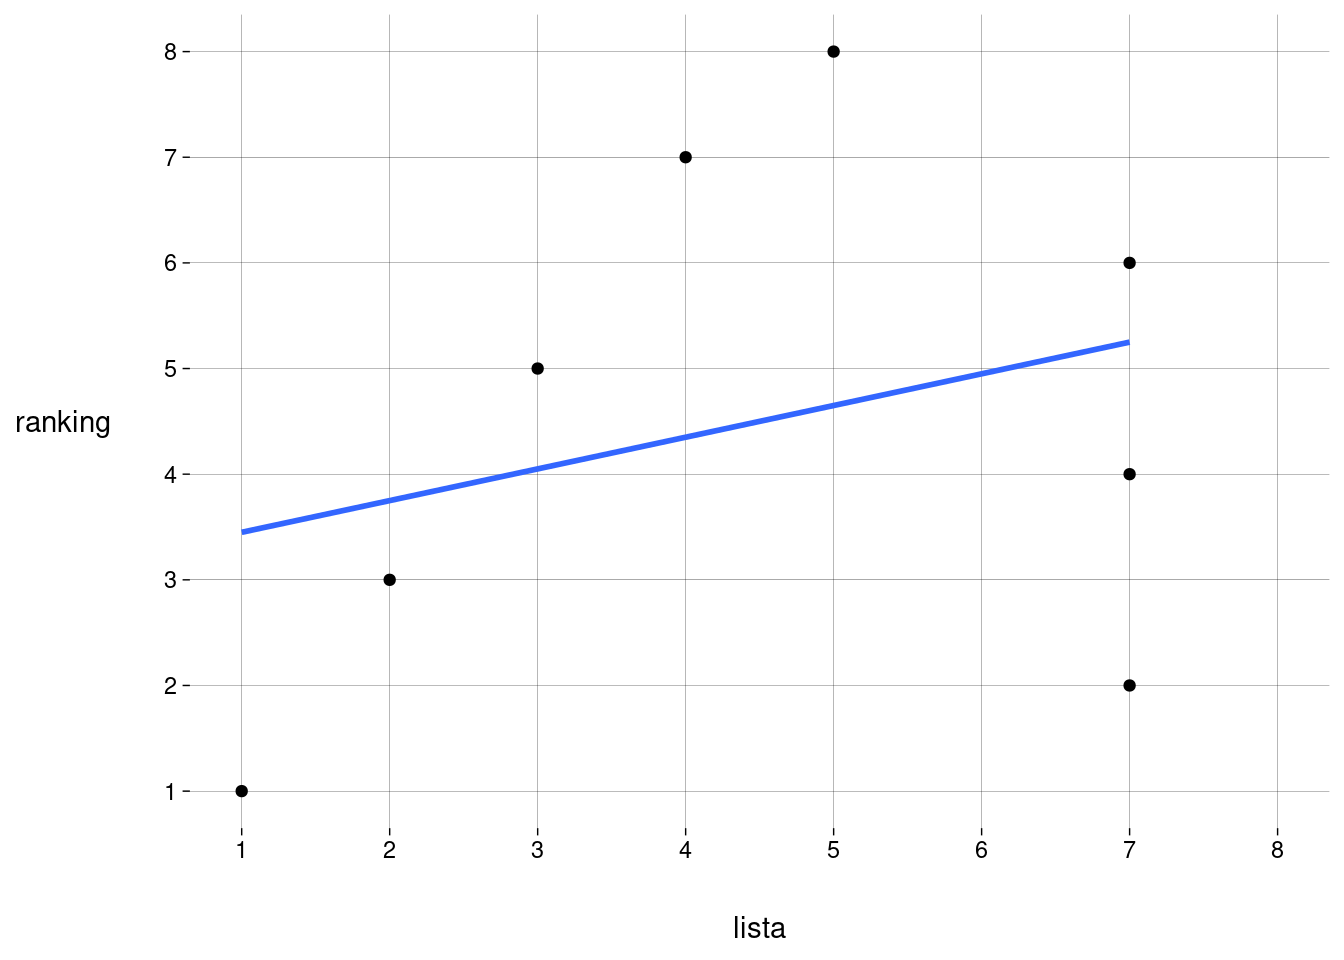
\includegraphics[width=1\textwidth,height=\textheight]{gerar-listas-e-rankings_files/figure-pdf/unnamed-chunk-15-1.pdf}
\end{center}

\begin{Shaded}
\begin{Highlighting}[]
\FunctionTok{criar\_plot}\NormalTok{(r, }\AttributeTok{reta =} \ConstantTok{FALSE}\NormalTok{)}
\end{Highlighting}
\end{Shaded}

\begin{center}
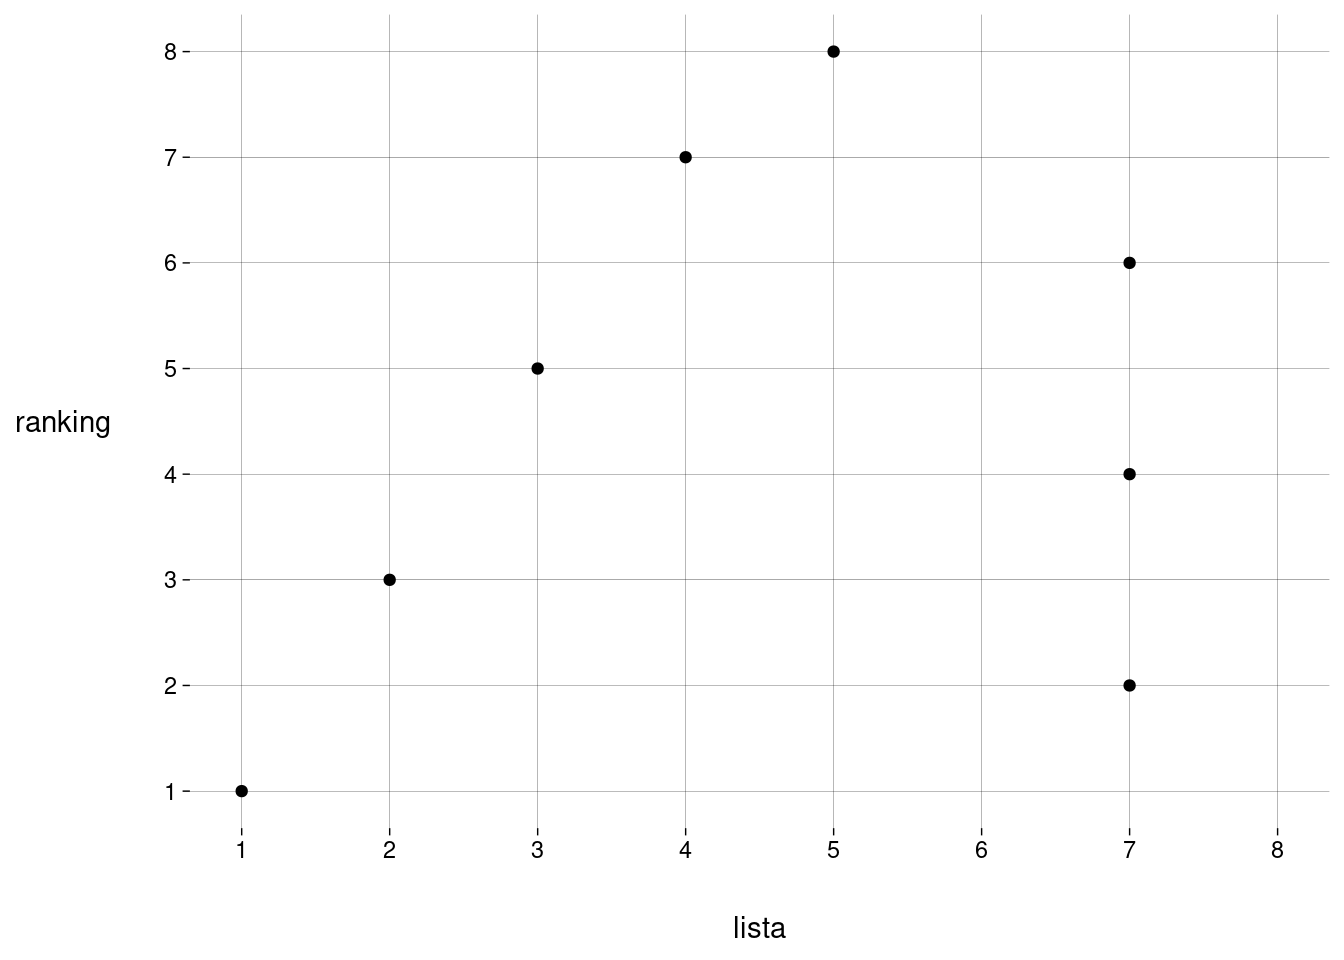
\includegraphics[width=1\textwidth,height=\textheight]{gerar-listas-e-rankings_files/figure-pdf/unnamed-chunk-16-1.pdf}
\end{center}

\begin{Shaded}
\begin{Highlighting}[]
\FunctionTok{criar\_plot}\NormalTok{(r, \textbackslash{}(df) \{ }\FunctionTok{cor}\NormalTok{(df}\SpecialCharTok{$}\NormalTok{pos\_lista, df}\SpecialCharTok{$}\NormalTok{pos\_ranking) }\SpecialCharTok{\%\textgreater{}\%} \FunctionTok{round}\NormalTok{(}\DecValTok{2}\NormalTok{) \})}
\end{Highlighting}
\end{Shaded}

\begin{center}
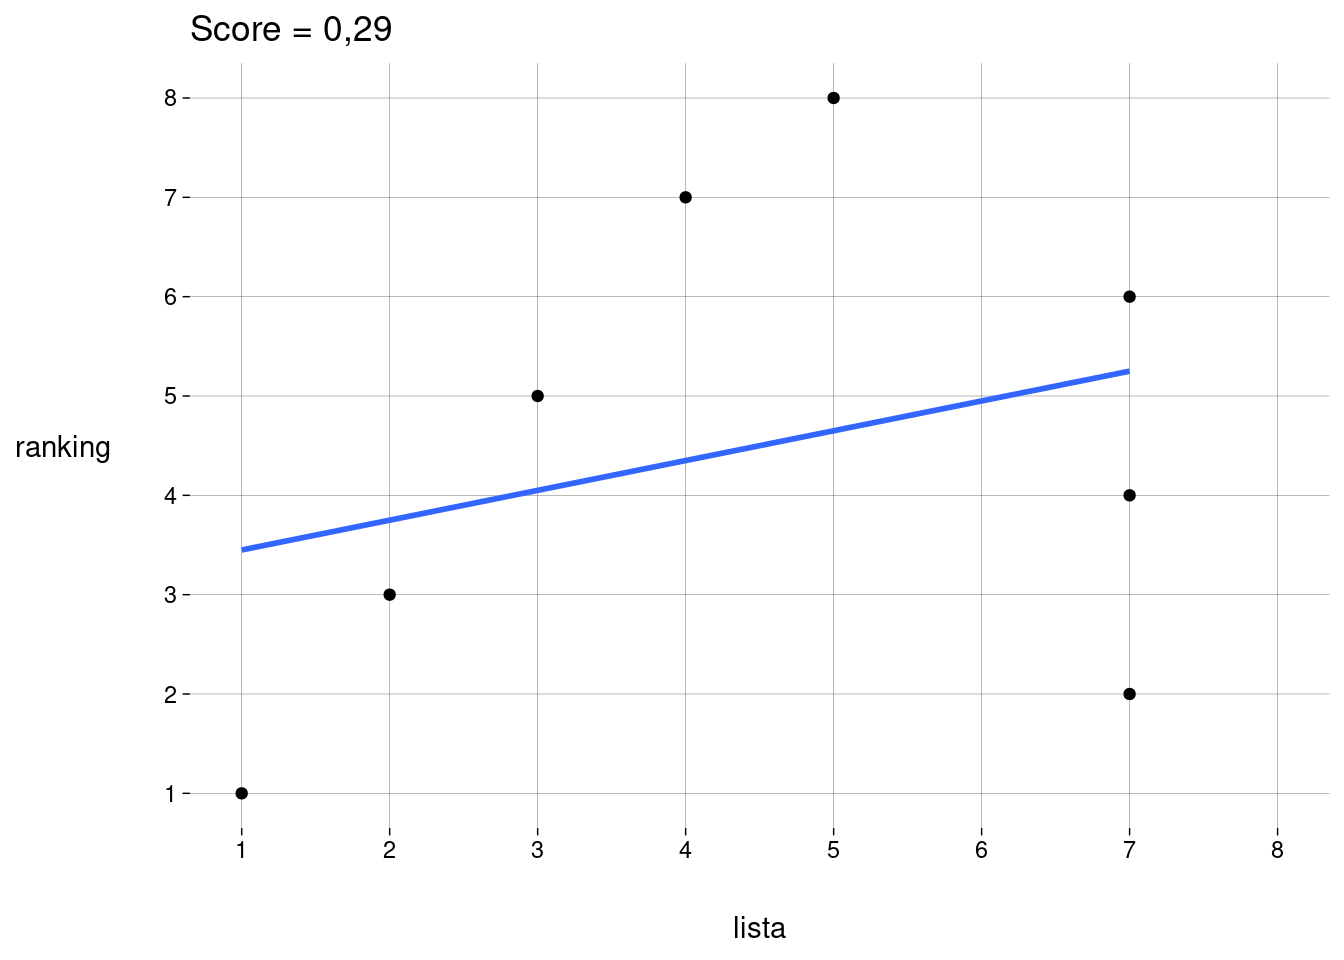
\includegraphics[width=1\textwidth,height=\textheight]{gerar-listas-e-rankings_files/figure-pdf/unnamed-chunk-17-1.pdf}
\end{center}

\subsection{\texorpdfstring{Criar uma tibble com todos os
\emph{rankings}}{Criar uma tibble com todos os rankings}}\label{criar-uma-tibble-com-todos-os-rankings}

Dados valores de $k$ e $p$, a função \texttt{criar\_df\_rankings()}
retorna uma \emph{tibble} com todos os $\binom{p - 1}{k - 1}$
\emph{rankings} possíveis.

Cada \emph{ranking} é representado por um \emph{string}, como descrito
na Seção~\ref{sec-repr}.

???



\end{document}
